Estabelecidos os requisitos pretendidos para a
implementação, foram atualizados os modelos conceptuais
de forma a sustentar as novas funcionalidades pretendidas.
\newline

\subsection{Gerador de Primitivas}

\begin{center}
    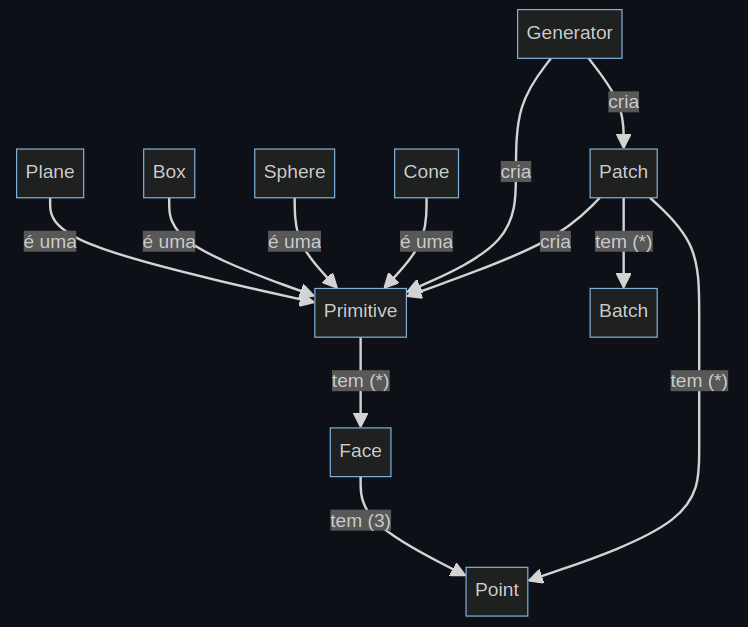
\includegraphics[width=0.8\textwidth]{imgs/concept1.png}
    \captionof{figure}{Modelo de Domínio do Gerador de Primitivas}
    \label{fig:domger}
\end{center}

\noindent
No gerador de primitivas as diferenças são mais notórias na parte
da implementação do que na arquitetura, visto que o maior papel
desta componente é realizar cálculos.\\
\\
Porém, ainda assim existem alguns componentes arquiteturais
que foram utilizados para auxiliar ao cálculo, armazenamento
e escrita das novas propriedades.\\
\\
O ponto do gerador passará, portanto, para além das suas coordenadas,
a armazenar também as coordenadas da sua normal, assim como, das
suas texturas, através da estrutura \textbf{TextureCoordinates}
(que será também utilizada para o motor gráfico).

\subsection{Motor gráfico}

\begin{center}
    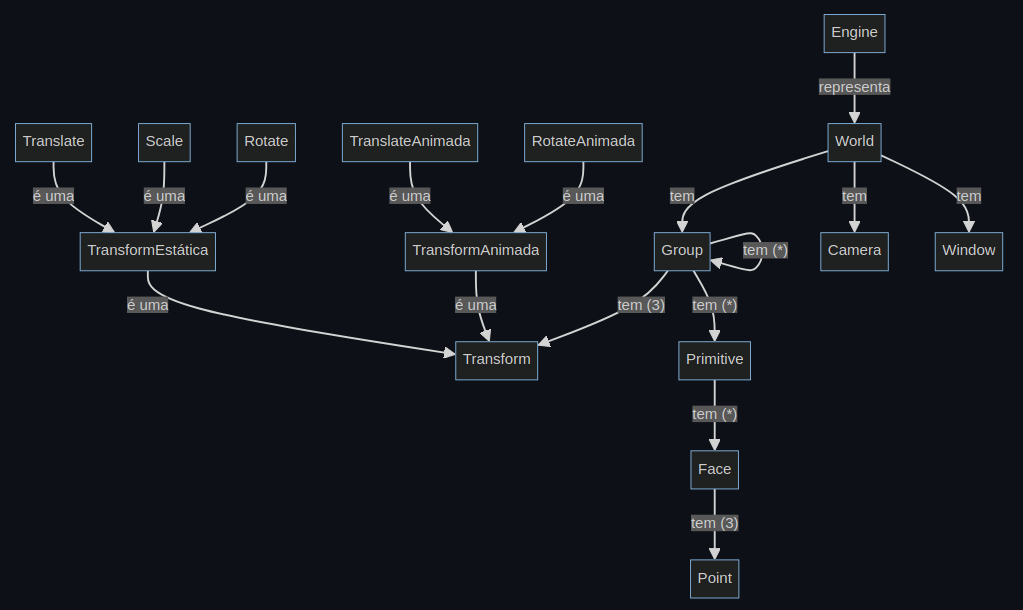
\includegraphics[width=1.0\textwidth]{imgs/concept2.png}
    \captionof{figure}{Modelo de Domínio do Motor Gráfico}
    \label{fig:domeng}
\end{center}

\noindent
Partindo da hierarquia até agora utilizada, o motor gráfico
teve algumas transformações notórias.\\
\\
Foram, portanto, esboçadas estruturas que suportem a definição
dos vários tipos de luz que deverão ser armazenadas num grupo
da configuração (como especificado nos requisitos).\\
\\
Estas estruturas conterão as propriedades necessárias para a
definição das luzes no cenário e deverão ser desenhadas após
as transformações do grupo serem aplicadas.\\
\\
Para além disso, deverão ser ativadas no início dos desenhos
do respetivo grupo e desativadas no final
do desenho do grupo (após o desenho dos sub-grupos), de forma
a cumprir o requisito e não
afetar outros grupos na mesma hierarquia.\\
\\
Ainda foram especificadas estruturas que pretendem armazenar
as componentes de cor e textura, pertencentes a uma primitiva.
A estrutura de cor é capaz de armazenar qualquer tipo de cor,
identificando o seu tipo nas suas propriedades e a estrutura
de textura guarda os índices necessários para a aplicação
de uma textura a um objeto.\\
\\
De forma a armazenar as normais, reutilizou-se a estrutura de
ponto, que, sendo constituída por três coordenadas e já ter
capacidade de leitura de ficheiros, rapidamente se encaixa
para este propósito. Para armazenar as coordenadas de textura,
reutilizou-se a estrutura já definida para o gerador.